\documentclass[12pt]{article}

\usepackage{amsmath}
\usepackage{amssymb}
\usepackage{geometry}
\usepackage{graphicx}
\usepackage{hyperref}

\geometry{letterpaper,tmargin=1in,bmargin=1in,lmargin=1in,rmargin=1in}

\hypersetup{
colorlinks, linkcolor=blue,
}


\begin{document}

\title{Analog Electronics}
\author{Laboratory exercise 4}
\date{Fall 2016}
\maketitle

\newpage
\section{Abstract}

In this experimentation using the information that was learned through lecture, we will design and construct a Difference Amplifier. This amplifier will be designed in Multi-Sim 13, and the majority of our calculations and testings will also be in Multi-Sim. The amplifier we design will be have a gain of $20v/v$. Once the designed amplifier meets all the design constraints, we will construct it using the given 741 op-amp and using our work bench tools; such as our occiliscope, function generator, multimeter, and our power supply. Once the circuit is constructed we then will test its various inputs and outputs to ensure our amplifier design meets the constraints given.

\section{Theory}

Multi-Sim is one of the most powerful tools an electrical engineer has at there disposal. By being able to create and test a circuit before spending time \& resources constructing it, we can work out problems before hand and ensure our specifications are met. By constructing the amplifier before hand  we can better understand the math and logic behind the difference amplifier and better understand how it works.

\newpage

\section{Experimentation}




This following image is the design of a difference amplifier made during the pre-lab. It will be used through the following experimentation. Keep in mind that during experimentation errors where found, primarily we will be using a $400k\Omega$ resistor in place of the $200k\Omega$ resistors.
\begin{figure}[h]
	\label{amp}
	\caption{Multi-Sim design of the Difference Amplifier}
	\centering
	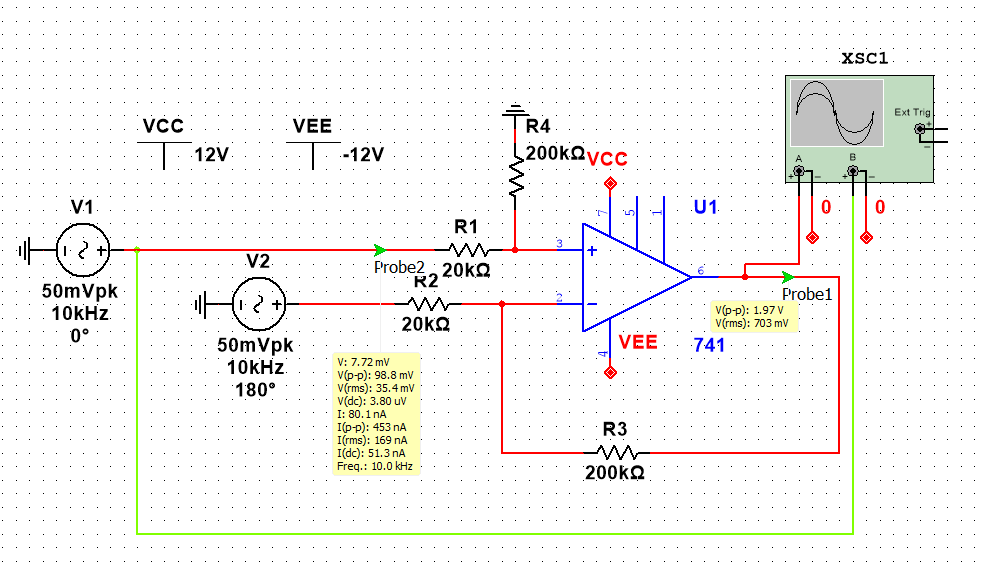
\includegraphics[width=1\textwidth]{amp}
\end{figure}



\newpage
\subsection{Setting up the Circuit \& DC source Voltage}
\begin{enumerate}
	\item Gather two $20k\Omega$,and 4 $200k\Omega$ resistors (You will use two of these as our $400k\Omega$ resistors.).
	\item Measure and log there values with the ohmmeter.
	\item Using Figure 1, build the circuit using the gathered resistors with your 741 op-amp.
	\item Ensure that the resistors go to the correct pins on our Op-Amp
	\item Attach your DC voltage to pins 7 and 4 as shown in the Figure 1
	\item Power the DC voltage source on.
	\item Using the DMM measure the input Voltage, the Inverting Voltage, and the Output Voltage.
	\item Log these values with your data.
\end{enumerate}

\subsection{Measuring DC gain of $V_1$ and $V_2$}

Now that we must use the circuit to measure the gain of both our inputs, $V_1$ \& $V_2$ 
\begin{enumerate}
	\item Ground our input $V_2$
	\item Attach a DC source to $V_1$
	\item $V_1$ value of $-2v$ to $2v$ with intervals of $.2v$, measure the output $V_o$ using the DMM
	\item Log this data into your table.
	
\end{enumerate}

To measure the DC gain of $V_2$ we will repeat the previous four steps, but this time we will ground $V_1$ and apply a DC voltage to $V_2$

\subsection{Measuring AC $V_1$ to $V_o$}

\begin{enumerate}
	\item Remove the DMM from the circuit.
	\item Attach a function generator with the corresponding sin wave as shown in figure 1.
	\item Using the Occiliscope compare and measure the waveforms of the input and the output.
	\item Log this data into your table.
	
\end{enumerate}
\newpage
\subsection{Measurements}

\begin{table}[!h]
	\centering
	\caption{OP-Amp only DC Voltage}
	\label{my-label}
	\begin{tabular}{ll}
		Input     & -1.8mV \\
		Output    & .001mV \\
		Inverting & -1.8mV
	\end{tabular}
\end{table}

\begin{table}[!h]
	\centering
	\caption{Measured Resistor Values}
	\label{my-label}
	\begin{tabular}{ll}
		398k  & 401k  \\
		19.7k & 19.8k
	\end{tabular}
\end{table}

\begin{table}[h!]
	\centering
	\caption{Input VS. Output Pk-Pk Voltages}
	\label{my-label}
	\begin{tabular}{ll}
		Input Vi & Output Vo \\
		0.05     & 0.92     
	\end{tabular}
\end{table}

\begin{table}[!h]
	\centering
	\caption{DC input measurements}
	\label{my-label}
	\begin{tabular}{llll}
		DC Voltage & $V_2$ Grounded & $V_1$ grounded & Both grounded \\
		-2   & -10.64 & 11.3   & 0.008 \\
		-1.8 & -10.64 & 11.3   & 0.008 \\
		-1.6 & -10.64 & 11.3   & 0.008 \\
		-1.4 & -10.64 & 11.3   & 0.008 \\
		-1.2 & -10.64 & 11.3   & 0.008 \\
		-1   & -10.64 & 11.3   & 0.008 \\
		-0.8 & -10.64 & 11.3   & 0.008 \\
		-0.6 & -10.64 & 11.3   & 0.008 \\
		-0.4 & -7.99  & 8      & 0.008 \\
		-0.2 & -3.99  & 4.01   & 0.008 \\
		0    & 0.006  & 0.008  & 0.008 \\
		0.2  & 4      & -3.99  & 0.008 \\
		0.4  & 8      & -7.98  & 0.008 \\
		0.6  & 11.3   & -10.64 & 0.008 \\
		0.8  & 11.3   & -10.64 & 0.008 \\
		1    & 11.3   & -10.64 & 0.008 \\
		1.2  & 11.3   & -10.64 & 0.008 \\
		1.4  & 11.3   & -10.64 & 0.008 \\
		1.6  & 11.3   & -10.64 & 0.008 \\
		1.8  & 11.3   & -10.64 & 0.008 \\
		2    & 11.3   & -10.64 & 0.008
	\end{tabular}
\end{table}


\newpage
\subsection{Post-Lab Calculations}
Now using our measurements we can calculate $A_{cm}$ \& $A_d$. To get these values we need to first find $V_cm$ \& $V_d$ respectively; we can find them with the following equations.

$$
V_{cm} = \frac{V_1 + V_2}{2} \qquad V_d = V_1 - V_2
$$
$$V_{cm}= \frac{.2V + 0}{2} = .1V \qquad V_d =.2V - 0V = .2V$$
Now we take these values and plug them into the equation for $A_{cm}$.

$$A_{cm} =\frac{V_{out}}{V_{cm}} = \frac{-3.99}{.1} = -39.95$$

To find $A_d$ we use the following equation.

$$A_d = \frac{V_{out}}{V_d} = \frac{-3.99}{.2} = -19.95$$

Now we can calculate the Common Mode Rejection Ratio as defined by,
 
$$CMRR = 20 \log \frac{A_d}{A_{cm}} = - 6 \ dB$$






\section{Conclusion}

In this experimentation we used a variety of analysis techniques to calculate and design an amplifier that took two input voltages and amplified them for a total of $20v/v$. During experimentation several problems occurred. First off, my initial plan of a ratio of 1:20 for resistor values was invalid, the method that was used in the end was a ratio of 1:40. This was due in fact that my simulated amplification was $20v/v$ for the combination of both inputs, in reality both channel was amplified by only ten. To fix this I had to make effort to ensure both channels received an input of $20v/v$. The second problem that arouse was the interval on which we measured our DC $V_o$, the interval range that was given was much to large and hit a maximum due to our amplifier only supplying +-12v . Overall the experiment was a success and it helped illustrate yet another use of the 741 amplifier.

\newpage
\section{Graph}
\begin{figure}[h]
	\label{amp}
	\caption{}
	\centering
	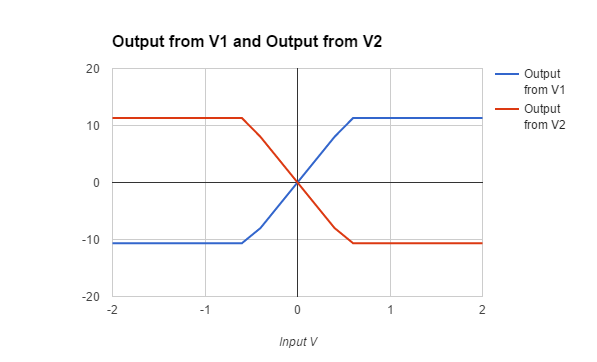
\includegraphics[width=1\textwidth]{graph}
	\end{figure}
\end{document}
